\section{Determining unstable operating performance points}
\label{sec:unstableOPPs}

We want to determine which OPPs are stable, and which OPPs are unstable, i.e.
those for which the system operates normally, and those which cause the system
to crash, respectively. Such a crash typically manifests as a kernel panic.
In particular, we would like to know which specific OPP lies on the boundary
between the stable realm and the unstable realm. Henceforth, such an OPP is
referred to as a \emph{crtitical point}. The following basic process lays out
how we can determine these critical points.

\begin{enumerate}
    \item Choose a frequency from the set of possible frequencies, and set that
        as the current CPU frequency.
    \item Decrease the CPU voltage by the smallest possible amount
        (i.e. $\frac{1}{1024}$ volts).
    \item Perform some fixed computational task, e.g. compute the SHA-1 hash of
        some predefined data. If the system crashes, record the current
        OPP as a critical point; else, go to step (2).
    \item Go to step (1), choosing a previously unchosen frequency if one
        exists; else, we have determined all the critical points.
\end{enumerate}

In practice, we expand upon this process in order to collect a more suitable
dataset. The process given above is repeated numerous times for each possible
frequency in order to obtain a reasonable sample size from which to determine
an average voltage offset which renders the system unstable. To save time in
collecting this data, we narrow down the range in which the critical point lies
for a given frequency by only testing certain OPPs, and then take the time to
more precisely find the critical point by testing all OPPs within this narrower
range of voltage offsets. We do this with the aid of the \code{cpupower} and
\code{undervolt} utilities discussed in §\ref{sec:cpupower} and
§\ref{sec:undervolt}, respectively.

The \code{undervolt} utility expects voltage offsets to be expressed in
millivolts (mV, units of $\frac{1}{1000}$ volts) rather than the MSR interface's
expected units of $\frac{1}{1024}$ volts. It then rounds the given value in
millivolts to the nearest multiple of $\frac{1}{1024}$ volts, and writes the
appropriate value to the MSR. As such, the "smallest possible amount" mentioned
in step (2) of the process above is taken as 1 mV rather than $\frac{1}{1024}$
volts. The process we end up using is described by the flowchart in Figure
\ref{fig:data-collection-flowchart}.

\begin{figure}[!htb]
    \center{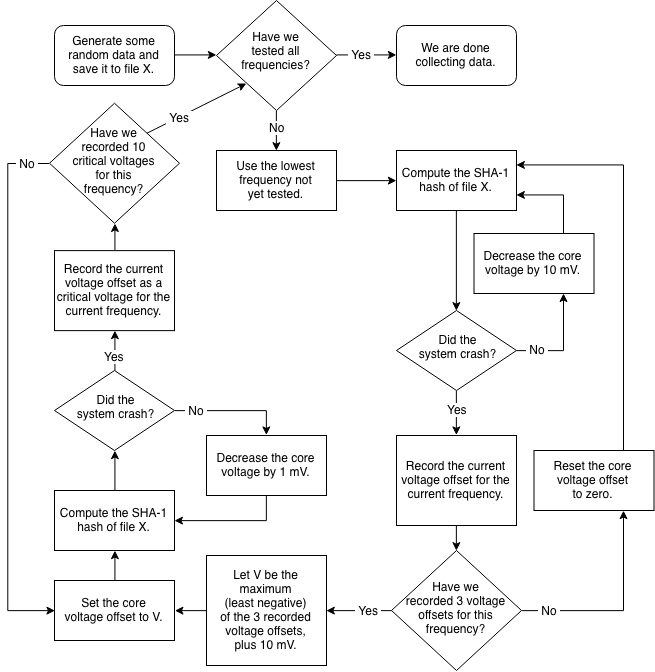
\includegraphics[width=\columnwidth,keepaspectratio]{data-collection-flowchart.png}}
    \caption{
        \label{fig:data-collection-flowchart}
        Flowchart describing how we collect data to determine the critical
        points.
    }
\end{figure}

In particular, we first find the critical point to the nearest 10 mV, performing
three (3) repetitions. We assume that the crticial point does not lie above the
maximum of these data points, plus another 10 mV for assurance. We then find the
critical point to as much accuracy as is possible (i.e. to the nearest 10 mV)
by testing every possible voltage offset within this narrower range, performing
ten (10) repetitions. We plot the mean, minimum, and maximum of these 10 data
points for each possible frequency in Figure \ref{fig:critical-points-graph}.
In this figure, the blue crosses are the mean voltage offset for each frequency.
The red diamonds are the bounds for the corrseponding error bars.

\begin{figure}[!htb]
    \center{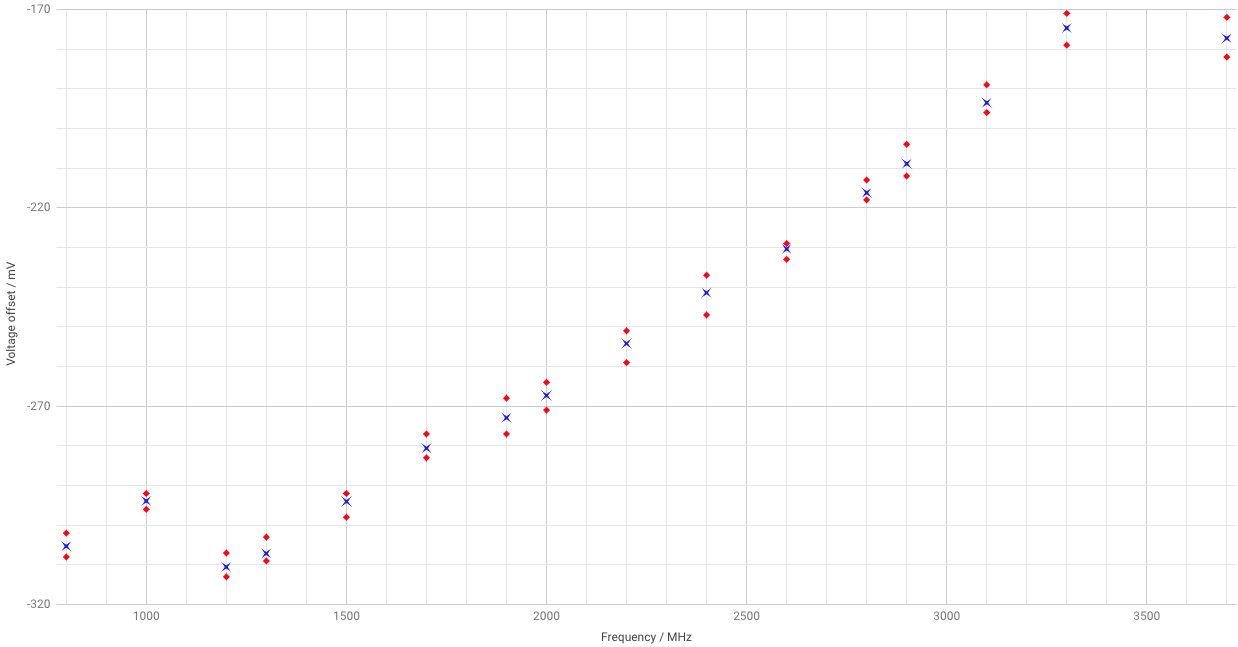
\includegraphics[width=\columnwidth,keepaspectratio]{critical-points-graph.png}}
    \caption{
        \label{fig:critical-points-graph}
        Graph plotting voltage offset against frequency for data points we have
        collected concerning critical points.
    }
\end{figure}

Ideally, this data collection would be automated, with the testbench running
through the process detailed above on boot, recording the tested OPPs to disk,
and rebooting after a system crash to repeat the process for different
frequencies as required. In practice, this is not possible, for the following
reasons:
\begin{itemize}
    \item any data that ought to be written to disk may not actually be flushed
        from memory to disk before the sytem encounters a kernel panic, 
        resulting in loss of these data; and
    \item the system does not always reboot after encountering a kernel panic,
        contrary to the operating system's intended function of rebooting 30
        seconds after a kernel panic. In such situations, the machine must be
        reset manually.
\end{itemize}

As such, we collect the data by hand with the aid of a shell script,
\code{undervolt-test.sh}, details of which are given in
§\ref{sec:undervolt-test.sh}.
